\section{Loss of Confidentiality in Counter Mode with Repeated Nonce}


When xoring two or more plaintexts with the same key it is possible two reproduce the plaintext by xor-ing two messages and trying common words. For English language words like "the" or "you" are very common and a good starting point.

Here we demonstrate the start of the process for Appendix B 1 and 2:\\

\begin{figure}[H]
	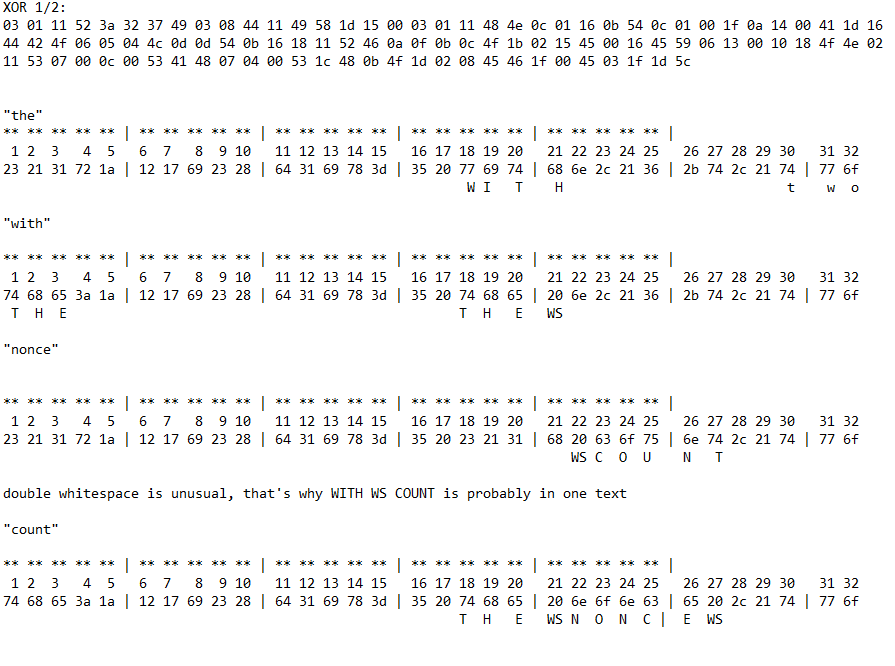
\includegraphics[width=1.0\textwidth]{Assignment0x03/images/xor_1_2}
\end{figure}

When we found all words, we got the sentence:\\
"Encrypting texts with counter mode is normally just fine, unless you do not take a fre" for chiphre 2.

By xoring that with the original chiphre text we got the key:

c9 3e 1e ba b7 3f c3 3c 05 a6 75 35 41 bd 34 5a e4 57 d1 a3 74 16 43 4e 02 3a 0b 0e d2 2b 9e 2c 32 c5 2a bb 75 5c 0b bf 54 29 2f 8e 63 53 b7 f3 45 b3 a5 c4 ee dd 4c 9a 03 da 4e 2b 2e 15 6b 80 7b ca 28 4c 9b 16 24 21 9b 1e 94 8f 51 59 d6 fb 5f 31 cb 06 f8 cc

Using this key, we can encrypt all messages by xoring the message with the key:

The PSI working Group congratulates you for solving this exercise. It was easy, right?\\
Encrypting texts with counter mode is normally just fine, unless you do not take a fre\\
For CBC mode, if the nonce is repeated, the attacker can only see if two messages have\\
No one should evEr use unauthenticated encryption, e.g. CTR or CBC without MAC, unless\\
If you authenticAte your ciphertext with a MAC, use the Encrypt then MAC construction\\
Given reasonable assumptions, the Encrypt then MAC construction was proven to be secur\\
The assumptions For the proof of security of Encrypt then MAC are a strongly unforgabl\\
There are cipher modes, which authenticate and encrypt in one step, without having to\\
One of the cipheR modes, which authenticate while encrypting is Galois Counter Mode, w\\
Galois Counter MOde (GCM) is very vulnerable to repeated nonces. You can even recover\\
Newer stream cipHers, e.g. NORX, use a duplex sponge construction to encrypt and authe\\

\paragraph{Suppose you were allowed to ask an oracle to encrypt any plaintext you like with the same nonce and key as used for the ciphertexts. For which plaintext would you like to obtain the ciphertext to get the keystream immediately?}

We would ask the oracle to encrypt one of the ciphertexts. This way we would receive the unencrypted plaintext and by xoring that plaintext with the corresponding ciphretext we would receive the key.
